\documentclass{article}%
\usepackage[T1]{fontenc}%
\usepackage[utf8]{inputenc}%
\usepackage{lmodern}%
\usepackage{textcomp}%
\usepackage{lastpage}%
\usepackage[head=40pt,margin=0.5in,bottom=0.6in]{geometry}%
\usepackage{graphicx}%
%
\title{\textbf{ONU quiere enfocar esfuerzos regionales en protección de migrantes venezolanos}}%
\author{AFP}%
\date{07/10/2018}%
%
\begin{document}%
\normalsize%
\maketitle%
\textbf{URL: }%
http://www.eluniversal.com/politica/22549/onu{-}quiere{-}enfocar{-}esfuerzos{-}regionales{-}en{-}proteccion{-}de{-}migrantes{-}venezolanos\newline%
%
\textbf{Periodico: }%
EU, %
ID: %
22549, %
Seccion: %
politica\newline%
%
\textbf{Palabras Claves: }%
NO\_TIENE\newline%
%
\textbf{Derecho: }%
18%
, Otros Derechos: %
CONTEXTO%
, Sub Derechos: %
NO\_TIENE%
\newline%
%
\textbf{EP: }%
NO\newline%
\newline%
%
\textbf{\textit{Queremos "que los venezolanos puedan tener instrumentos, acceso a una protección en varios países y que no sean expuestos a riesgos, a criminalidad, y peligros", sostuvo Filippo Grandi}}%
\newline%
\newline%
%
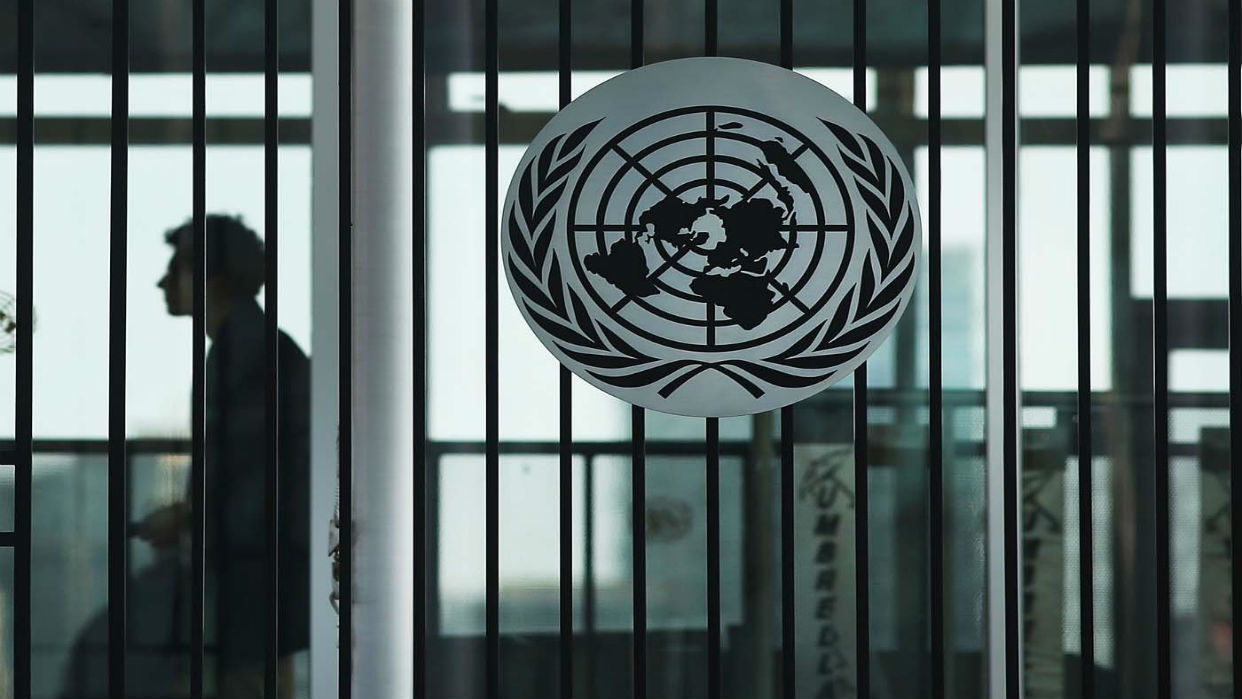
\includegraphics[width=300px]{96.jpg}%
\newline%
%
Bogota{-} El Alto Comisionado de la ONU para los Refugiados, Filippo Grandi, afirmó a su llegada a Colombia que se enfocará en la protección regional de los migrantes venezolanos para evitar que sean víctimas de la criminalidad, especialmente las mujeres y los niños.%
\newline%
%
Grandi, quien inició una gira que también lo llevará por Argentina, Perú y Ecuador, aseguró a la prensa que su "mayor preocupación" son los riesgos que están enfrentando los venezolanos que huyen en masa de la crisis económica en el país petrolero.%
\newline%
%
Queremos "que los venezolanos puedan tener instrumentos, acceso a una protección (...) en varios países y que no sean expuestos a riesgos, a criminalidad, peligros, especialmente las mujeres, los niños", sostuvo el funcionario de Naciones Unidas.%
\newline%
%
Grandi anunció ayer que viajará este domingo a la ciudad fronteriza de Cúcuta {-}por donde ingresan los venezolanos que en un importante número siguen su travesía hacia el sur del continente{-}, para "ver personalmente" la situación.%
\newline%
%
El Alto Comisionado para los Refugiados insistió en que este inusual éxodo {-}que el Gobierno de Nicolás Maduro niega{-} debe atenderse mediante "una estrategia regional, porque muchos problemas son los mismos en diferentes países", reseñó AFP.%
\newline%
%
En ese sentido, destacó la reciente designación del exvicepresidente de Guatemala Eduardo Stein como su representante para los migrantes y refugiados de Venezuela. \newline%
\newline%
"Su papel será el de coordinar la acción internacional de manera más eficaz, de buscar recursos, más recursos para ayudar a los venezolanos", señaló.%
\newline%
%
La ONU calcula que cerca de 1,9 millones de personas han dejado Venezuela desde 2015, a causa de la difícil situación interna marcada por la escasez de alimentos y medicinas y productos básicos, además de una hiperinflación.%
\newline%
%
Solo Colombia estima un flujo migratorio de un millón de personas por su territorio, y ha regularizado temporalmente a 820 mil venezolanos.%
\newline%
%
En una reciente declaración en Ginebra, Grandi precisó que "unas 5.000 personas abandonan Venezuela cada día actualmente", en "el mayor movimiento de población en la historia reciente de América Latina".%
\newline%
%
El presidente de Venezuela niega que en su país haya una crisis migratoria y ha pedido a la ONU "sincerar" las estadísticas. \newline%
\newline%
También desmiente que exista una emergencia humanitaria a raíz de la escasez crónica de artículos de primera necesidad.%
\newline%
%
Antes de proseguir su periplo por Argentina, Grandi se reunirá el lunes con el presidente de Colombia, Iván Duque, quien desde su llegada al poder el 7 de agosto está ejerciendo una fuerte presión diplomática sobre Maduro, a cuyo gobierno tacha de "dictadura".%
\newline%
%
\end{document}